\chapter{Nonlinear Time Reversal}
\label{ch:nltr}

The preceding chapters have been concerned with linear time reversal, or LTR, and have focused primarily on investigating properties of reconstructions. Now, we move into our nonlinear(NLTR) investigations, which focus on proof of concept of targeting capabilities. NLTR makes use of harmonic reflections from the target to isolate it via frequency domain inspection after the sona is collected, a process similar to how we would envision a TR based WPT system to work.

Conceptually, our general process is this: we broadcast a Gaussian pulse from one port. Elsewhere in the cavity is a nonlinear element serving as a target. Any signal that interrogates this element will generate higher frequency harmonics of the interrogation signal. These harmonics are embedded along with all the other echoes in the sona collected back at the transceiving port. However, before time reversing the sona, we transform it into the frequency domain and filter out all the components not within some band of the harmonic frequencies. In this way, we isolate only those wave paths that had contact with the nonlinear target. That filtered sona is time reversed and rebroadcast from the transceiving port, which will cause a slightly distorted version of the original Gaussian pulse to reconstruct at the target. This process is illustrated in Figure~\ref{fig:nonlinear-diagram}.

\begin{figure}[]
\centering
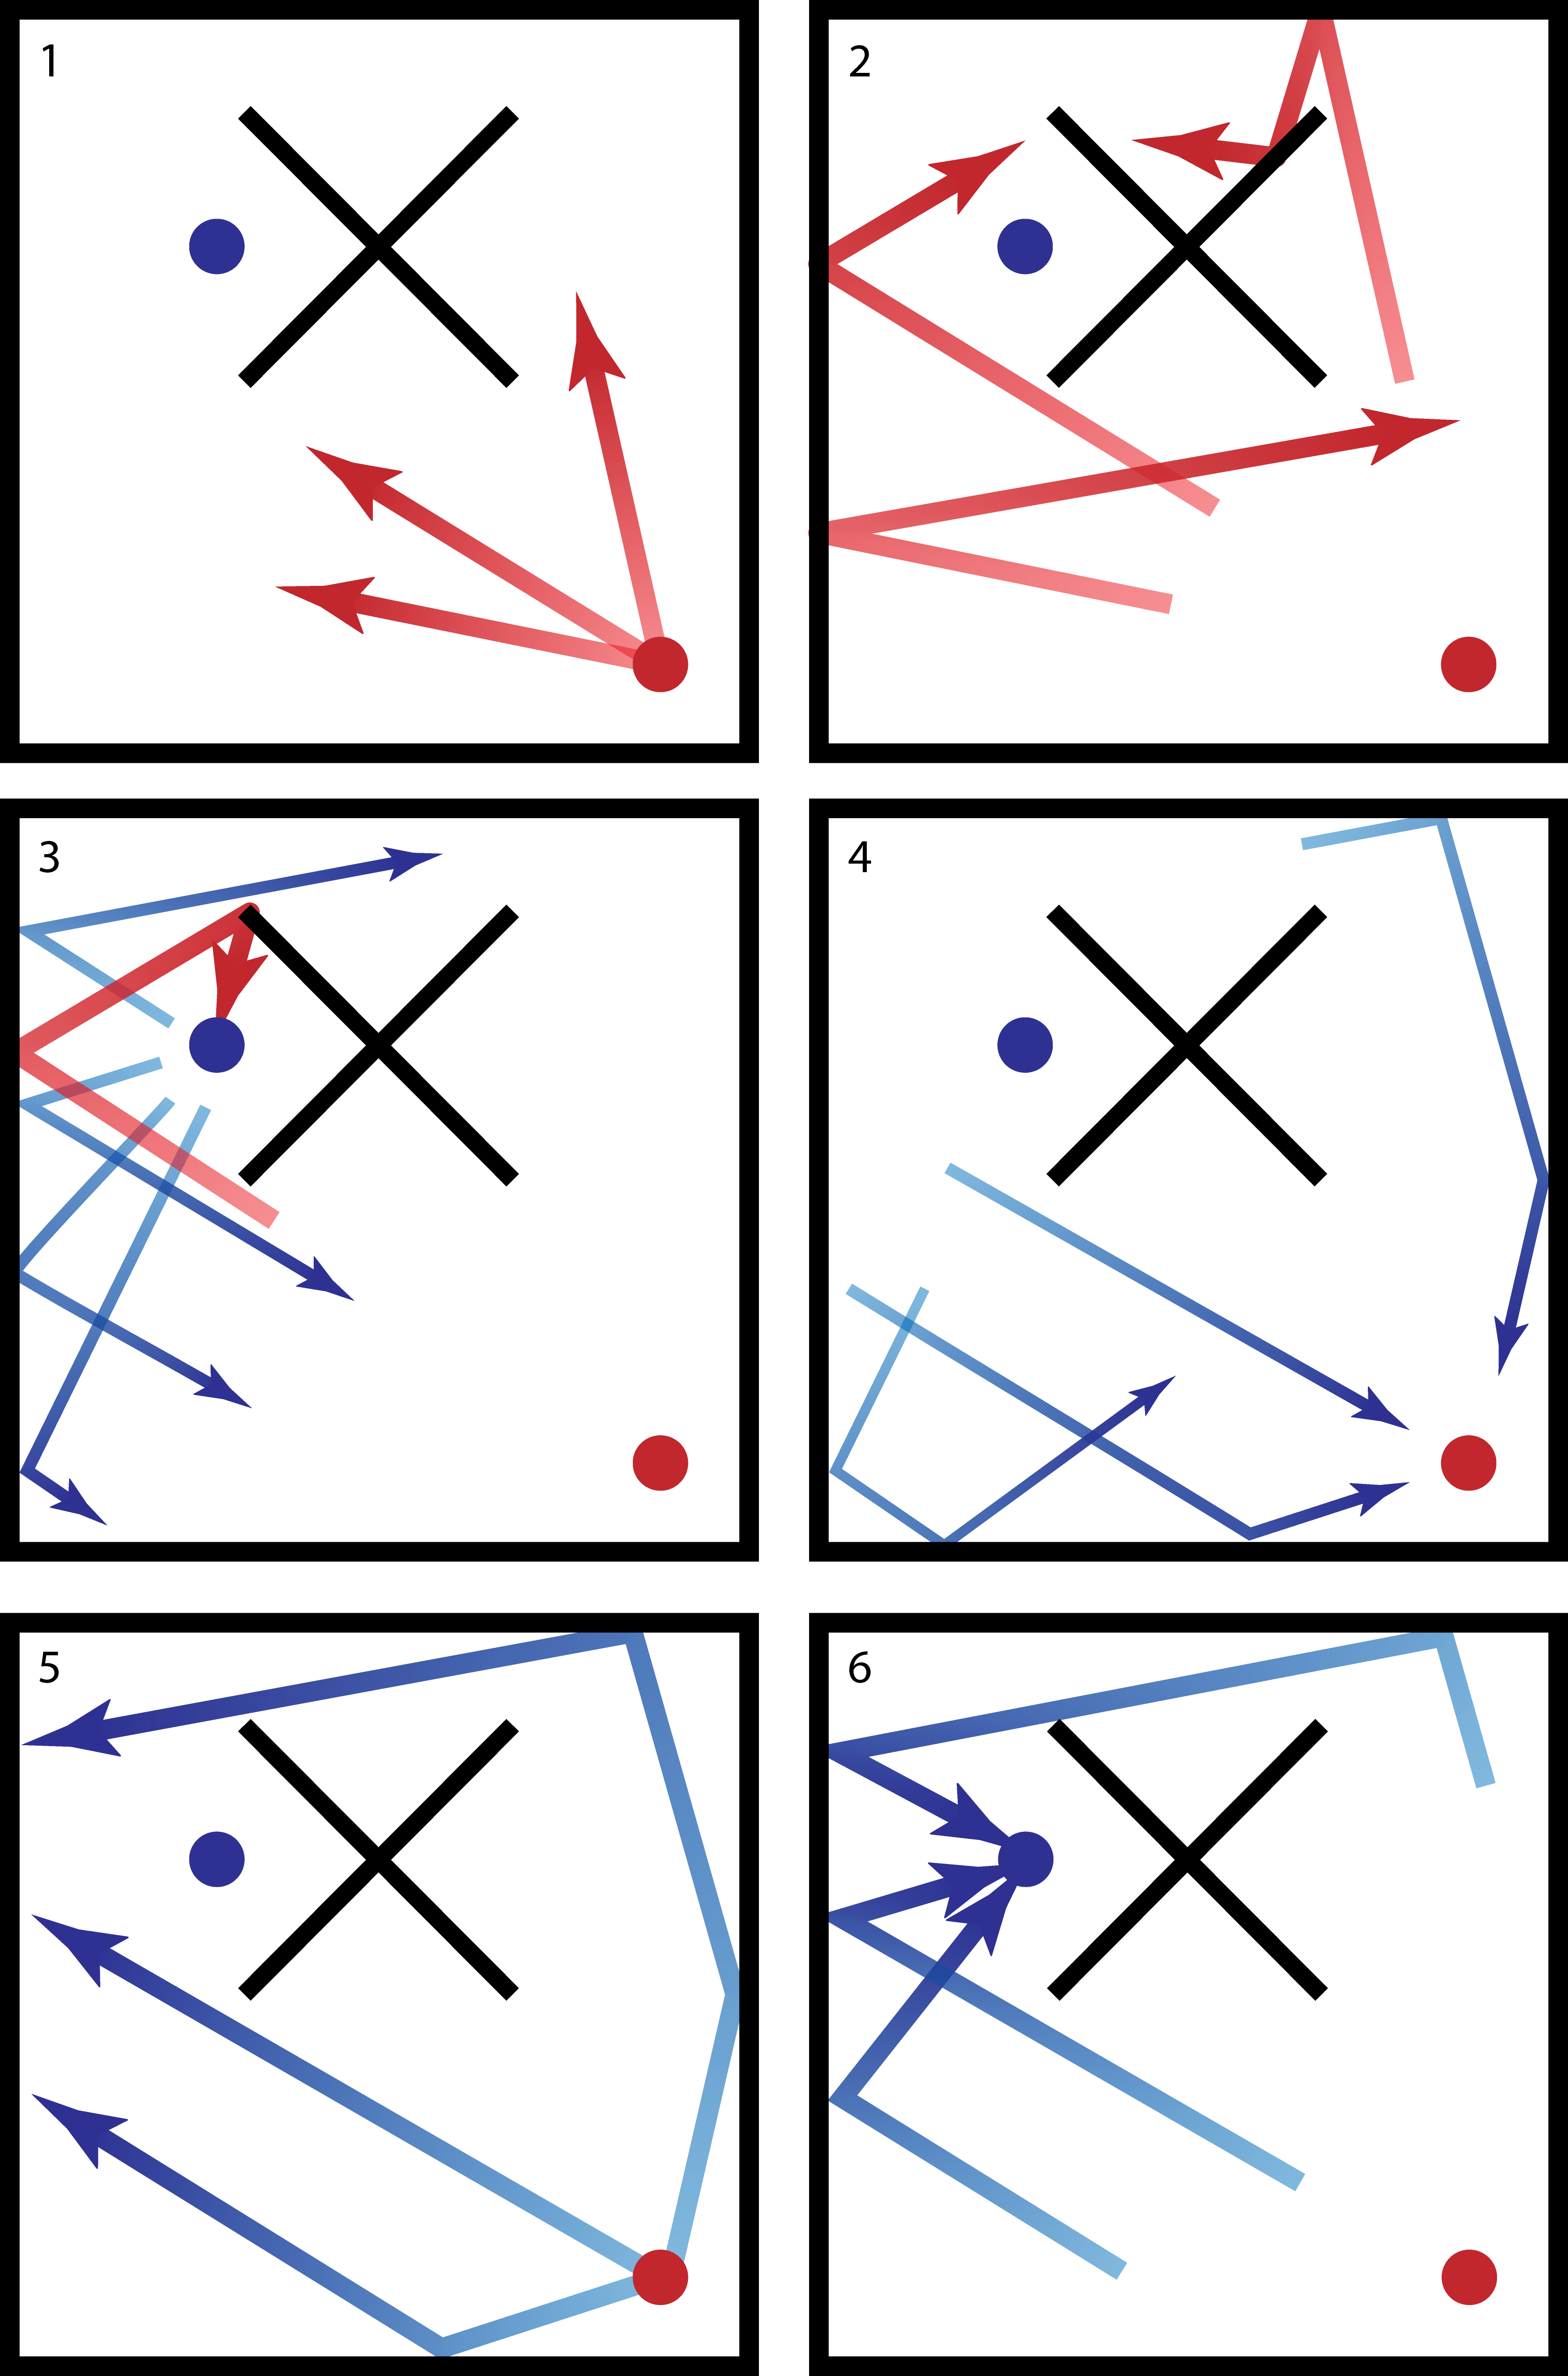
\includegraphics[width=0.7\textwidth]{nonlinear/diagram}
    \caption[Conceptual overview of nonlinear time reversal]{Reading order from top left: (1) The TRM broadcasts a signal into the cavity at one frequency, which (2) reverberates within the cavity. Eventually, (3) the signal reaches the nonlinear element somewhere within the chamber. Reflected waves that encounter this element have a characteristic frequency signature containing harmonics of the original signal. (4) Some of these harmonic reflections find their way back to the TRM. The TRM filters the sona to extract only those reflections, then time reverses and (5) re-emits them. (6) The time reversed waves collapse back on the nonlinear target.}
    \label{fig:nonlinear-diagram}
\end{figure}

We explored several different applications of NLTR with an eye towards adapting the technique for WPT, both experimentally and in simulation. The experimental portions met with limited success due to the difficulty of passively producing harmonics of significant magnitude. We attempted to use both a diode as an electric nonlinear object due to its nonlinear I-V curve as well as ferromagnetic nanorods as a magnetically nonlinear object due to the nonlinear magnetization curve. In both instances, the nonlinear response we obtained was quite small. Due to this limitation, our NLTR experiments took place entirely within the realm of numerical simulations.
